\section{锥的同调}
\sourcepage{51--52}
现在计算 $n$ 维单形及其边界的同调。为方便起见，先引入锥的概念。

\entry{定义}{1.9.1}设 $K$ 是 $E^J$ 中的复形，$w\in E^J$，且从 $w$ 出发的每条射线与 $|K|$ 至多相交于一点。定义\textbf{以 $w$ 为顶点的 $K$ 上的锥}（cone），为所有形如 $wa_0a_1\cdots a_p$ 的单形及其所有面构成的族，其中 $a_0a_1\cdots a_p$ 为 $K$ 的单形。记作 $w*K$，见图 1.9.1。\translatornote{锥的这一几何构造还需假定 $w\notin|K|$；原文未单独明说。}
\begin{center}
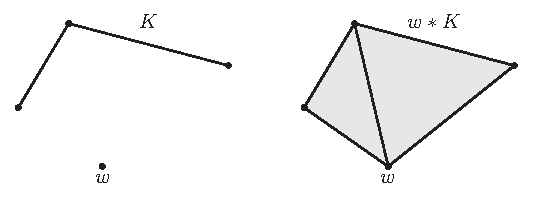
\includegraphics[width=96mm]{figures/1-9-1.pdf}\\图 1.9.1
\end{center}
下面说明 $w*K$ 是良定义的复形，并包含 $K$ 为子复形。$K$ 常称为锥的\textbf{底}（base）。

先证明点集 $\{w,a_0,a_1,\ldots,a_p\}$ 几何独立。若 $w$ 位于 $a_0,\ldots,a_p$ 确定的平面 $P$ 中，考察连接 $w$ 与 $\sigma=a_0\cdots a_p$ 的内点 $x$ 的线段。由于 $\Int\sigma$ 在 $P$ 中开，它包含这条线段上的一个区间。但根据假设，从 $w$ 经过 $x$ 的射线与 $|K|$ 只有一个交点，矛盾。

再证明 $w*K$ 是复形。其单形有三类：$K$ 的单形 $a_0\cdots a_p$，形如 $wa_0\cdots a_p$ 的单形，以及 $0$ 维单形 $w$。第一类的不同单形内部不交，因为 $K$ 是复形。开单形 $\Int(wa_0\cdots a_p)$ 是连接 $w$ 与 $\Int(a_0\cdots a_p)$ 中各点的所有开线段的并；这样的两个开单形不能相交，因为从 $w$ 出发的任何射线都不会包含 $|K|$ 中多于一个点。同理，第一类与第二类单形的内部也不相交。

\entry{例}{1.9.2}设 $K_\sigma$ 是由单形 $\sigma=v_0v_1\cdots v_n$ 及其各面组成的复形，则 $K_\sigma=v_0*K_s$，其中 $s$ 是 $\sigma$ 中与 $v_0$ 相对的面。因此，每个正维单形都是锥。

\entry{例}{1.9.3}设 $K$ 是 $\R^2$ 中由 $x$ 轴上的区间 $[n,n+1]\times0$ 及其顶点组成的复形，$w$ 是 $y$ 轴上不同于原点的一点。则 $w*K$ 为图 1.9.2 的复形。虽然 $|K|$ 是 $\R^2$ 的子空间，$|w*K|$ 却不是，见第 1.3 节习题 9。
\begin{center}
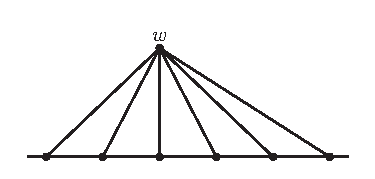
\includegraphics[width=68mm]{figures/1-9-2.pdf}\\图 1.9.2
\end{center}
锥构造的一个特别有用的推论如下。

\entry{引理}{1.9.4}设 $U$ 是 $\R^n$ 中的有界凸开集，$w\in U$。若 $K$ 是满足 $|K|=\overline U\setminus U$ 的有限复形，则 $w*K$ 为有限复形，且 $|w*K|=\overline U$。

\noindent\textbf{证明：}由引理 1.2.7，从 $w$ 出发的每条射线与 $|K|$ 恰好相交于一点，而且 $\overline U$ 是连接 $w$ 与 $|K|$ 中各点的所有线段的并。\hfill$\square$

\sourcepage{53}
给定 $K$，其上的任意两个锥 $w*K$、$z*K$ 同构：将 $K$ 的各顶点映到自身，并将 $w$ 映到 $z$ 的顶点映射，诱导了这两个锥之间的同构。

注意，对于 $\R^N$ 中的复形 $K$，可能不存在 $\R^N$ 中的点 $w$ 使锥 $w*K$ 能够构成。不过，总可以将 $K$ 视为 $\R^N\times0\subset\R^{N+1}$ 中的复形，此时取 $w=(0,0,\ldots,0,1)\in\R^{N+1}$ 即可。对 $E^J$ 中的复形也有类似结论。

下面计算锥的同调，证明其正维同调均为零。为此引入一种括号运算，后文也将用到。

\entry{定义}{1.9.5}设 $w*K$ 为锥。若 $\sigma=[a_0,a_1,\ldots,a_p]$ 是 $K$ 的定向单形，以 $[w,\sigma]$ 表示 $w*K$ 的定向单形 $[w,a_0,a_1,\ldots,a_p]$。此运算良定义：交换序列 $[a_0,\ldots,a_p]$ 中两个顶点，恰好也交换 $[w,a_0,\ldots,a_p]$ 中两个顶点。更一般地，若 $c_p=\sum n_i\sigma_i$ 是 $K$ 的 $p$ 维链，定义
\[
[w,c_p]=\sum n_i[w,\sigma_i].
\]
这个括号运算是将 $C_p(K)$ 映入 $C_{p+1}(w*K)$ 的同态。\translatornote{原文将目标写作 $C_{p+1}(K)$，但加上顶点 $w$ 后的单形属于锥 $w*K$。}
由边界公式容易计算：
\[
\partial[w,\sigma]=\begin{cases}
\sigma-w,&\dim\sigma=0,\\
\sigma-[w,\partial\sigma],&\dim\sigma>0.
\end{cases}
\]
从而得到更一般的公式：
\[
\partial[w,c_0]=c_0-\epsilon(c_0)w,\qquad
\partial[w,c_p]=c_p-[w,\partial c_p]\quad(p>0).
\]
\entry{定理}{1.9.6}若 $w*K$ 是锥，则对所有 $p$ 都有 $\widetilde H_p(w*K)=0$。

一般地，若复形在所有维数上的约化同调都为零，就称其为\textbf{无环的}（acyclic）。

\sourcepage{54}
\noindent\textbf{证明：}由于 $|w*K|$ 连通，其零维约化同调为零。设 $p>0$，取 $w*K$ 的 $p$ 维闭链 $z_p$，证明它是边界。写作
\[
z_p=c_p+[w,d_{p-1}],
\]
其中 $c_p$ 由 $z_p$ 中那些由 $K$ 承载的项组成，$d_{p-1}$ 为 $K$ 的链。只需证明 $z_p-\partial[w,c_p]=0$。直接计算得
\[
\begin{aligned}
z_p-\partial[w,c_p]
&=c_p+[w,d_{p-1}]-c_p+[w,\partial c_p]\\
&=[w,e_{p-1}],
\end{aligned}
\]
其中 $e_{p-1}=d_{p-1}+\partial c_p$ 是 $K$ 的链。\translatornote{原文定义该链时左端下标印作 $e_p$，据维数与后文应为 $e_{p-1}$。}因为 $z_p$ 是闭链，对上式取边界得
\[
0=\begin{cases}
e_{p-1}-\epsilon(e_{p-1})w,&p=1,\\
e_{p-1}-[w,\partial e_{p-1}],&p>1.
\end{cases}
\]
这个链中由 $K$ 承载的部分只有 $e_{p-1}$，故 $e_{p-1}=0$。所以
\[
z_p-\partial[w,c_p]=[w,e_{p-1}]=0,
\]
得到所需结论。\hfill$\square$

\entry{定理}{1.9.7}设 $\sigma$ 为 $n$ 维单形，则由 $\sigma$ 及其各面构成的复形 $K_\sigma$ 无环。若 $n>0$，令 $\Sigma^{n-1}$ 为多胞体等于 $\Bd\sigma$ 的复形，并给 $\sigma$ 定向。则 $\widetilde H_{n-1}(\Sigma^{n-1})$ 为无限循环群，由链 $\partial\sigma$ 生成；当 $i\ne n-1$ 时，$\widetilde H_i(\Sigma^{n-1})=0$。

回顾引理 1.2.6，$\Bd\sigma$ 同胚于 $S^{n-1}$，所以此定理给出了球面的同调。

\noindent\textbf{证明：}由于 $K_\sigma$ 是锥，它无环，见例 1.9.2。\translatornote{此论证直接适用于 $n>0$；当 $n=0$ 时，$K_\sigma$ 是单点复形，其约化同调直接由定义为零。}比较 $K_\sigma$ 与 $\Sigma^{n-1}$ 的链群，除 $n$ 维外，它们相同。下图保留边界算子的维数下标，并区分两个复形的边界算子：
\[
\begin{array}{ccccccccc}
C_n(K_\sigma)&\xrightarrow{\partial_n}&C_{n-1}(K_\sigma)&\xrightarrow{\partial_{n-1}}&\cdots&\xrightarrow{\partial_1}&C_0(K_\sigma)&\xrightarrow{\epsilon}&\Z\\
&&\Vert&&&&\Vert&&\Vert\\
0&\xrightarrow{\partial'_n}&C_{n-1}(\Sigma^{n-1})&\xrightarrow{\partial'_{n-1}}&\cdots&\xrightarrow{\partial'_1}&C_0(\Sigma^{n-1})&\longrightarrow&\Z.
\end{array}
\]
立即得 $i\ne n-1$ 时，$\widetilde H_i(\Sigma^{n-1})=\widetilde H_i(K_\sigma)=0$。

\sourcepage{55--56}
再算 $n-1$ 维同调。先设 $n>1$。由于 $C_n(\Sigma^{n-1})$ 为平凡群，$C_{n-1}(\Sigma^{n-1})$ 中没有非零边界。于是
\[
\begin{aligned}
H_{n-1}(\Sigma^{n-1})&=Z_{n-1}(\Sigma^{n-1})\\
&=\ker\partial'_{n-1}=\ker\partial_{n-1}\\
&=\operatorname{im}\partial_n,
\end{aligned}
\]
最后一步因为 $H_{n-1}(K_\sigma)=0$。$C_n(K_\sigma)$ 为由 $\sigma$ 生成的无限循环群，所以 $\operatorname{im}\partial_n$ 是由 $\partial_n\sigma$ 生成的循环群；因为 $C_{n-1}(K_\sigma)$ 无挠，它为无限群。

$n=1$ 的论证类似，只需始终将 $\partial_{n-1}$ 换为 $\epsilon$。\hfill$\square$

下面的定义在习题中要用到；“悬挂”的概念也将在后面各节再次出现。

\entry{定义}{1.9.8}设 $K$ 为复形，$w_0*K$、$w_1*K$ 为其上的两个锥，且其多胞体仅在 $|K|$ 相交。习题 1(a) 要求证明 $(w_0*K)\cup(w_1*K)$ 是复形，称为 $K$ 的一个\textbf{悬挂}（suspension），记为 $S(K)$，见图 1.9.3。
\begin{center}
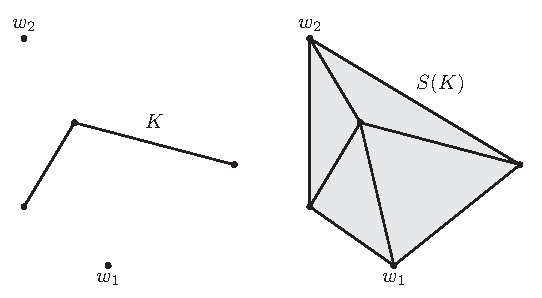
\includegraphics[width=98mm]{figures/1-9-3.pdf}\\图 1.9.3
\end{center}
\subsection*{习题}
\begin{enumerate}
\item 设 $K$ 为复形，$w_0*K$、$w_1*K$ 为两个多胞体仅在 $|K|$ 相交的锥。
\begin{enumerate}[label=(\alph*)]
\item 证明 $(w_0*K)\cup(w_1*K)$ 是复形。
\item 用括号记号，按公式 $\varphi(c_p)=[w_0,c_p]-[w_1,c_p]$ 定义 $\varphi:C_p(K)\to C_{p+1}(S(K))$。证明 $\varphi$ 诱导同态
\[
\varphi_*:\widetilde H_p(K)\longrightarrow\widetilde H_{p+1}(S(K)).
\]
\item 证明：若 $K$ 由一个 $2$ 维单形的所有真面组成，则 $\varphi_*$ 是同构。
\end{enumerate}
后面将看到，一般情况下 $\varphi_*$ 也是同构，见第 3.4 节。
\end{enumerate}
